\documentclass[a4paper, 11pt]{article}
\usepackage[utf8]{inputenc}
\usepackage[english]{babel}
\usepackage[utf8]{inputenc}
\usepackage[margin=2.cm]{geometry}
\usepackage{fancyhdr}

\usepackage[T1]{fontenc}
\usepackage{lmodern}

\usepackage{graphicx}
\graphicspath{ {images/} }
\usepackage{pdflscape}


\usepackage{array}

\usepackage{multirow}

\usepackage{color,array}

\definecolor{mygray}{gray}{0.6} %custom color for text

\usepackage{float}
\usepackage[table,xcdraw]{xcolor}


\usepackage{varwidth} %for lists next to each other

%for subfigure
\usepackage{subcaption}


%Includes "References" in the table of contents
\usepackage[nottoc]{tocbibind}

\usepackage{enumitem}
\setlist{nolistsep}


\fancypagestyle{plain}{%
  \renewcommand{\headrulewidth}{0pt}%
  \fancyhf{}%
  \fancyfoot[L]{\footnotesize Raymond Lochner}
  \fancyfoot[C]{\footnotesize December 2017 - Université libre de Bruxelles}%
  \fancyfoot[R]{\thepage}
}
\pagestyle{plain}

\date{\today}

\begin{document}

\begin{titlepage}
	\centering
	{\scshape\LARGE Université libre de Bruxelles \par}
	\vspace{1cm}
	{\scshape\Large INFO-F-409 - Learning Dynamics\par}
	\vspace{1.5cm}
	{\huge\bfseries {Assignment Three\par}}
	\vspace{0.5cm}
	{\Large Multi-Armed Bandits\par}
	\vspace{2cm}
	{\Large Raymond Lochner - 000443637\par}
	\vspace{0.5cm}
	{\Large raymond.lochner@ulb.ac.be}
	\vfill
	
	\setcounter{tocdepth}{2} %hides subsubsections in TOC
	\tableofcontents

\vfill
% Bottom of the page
	{\large \today \par}
\end{titlepage}

\newpage

\section*{Preliminary information}

Every experiment was run 2000 times and the results averaged

\section{Exercise 1}
\subsection{Combined Average Reward}

\begin{figure}[H]
	\centering
    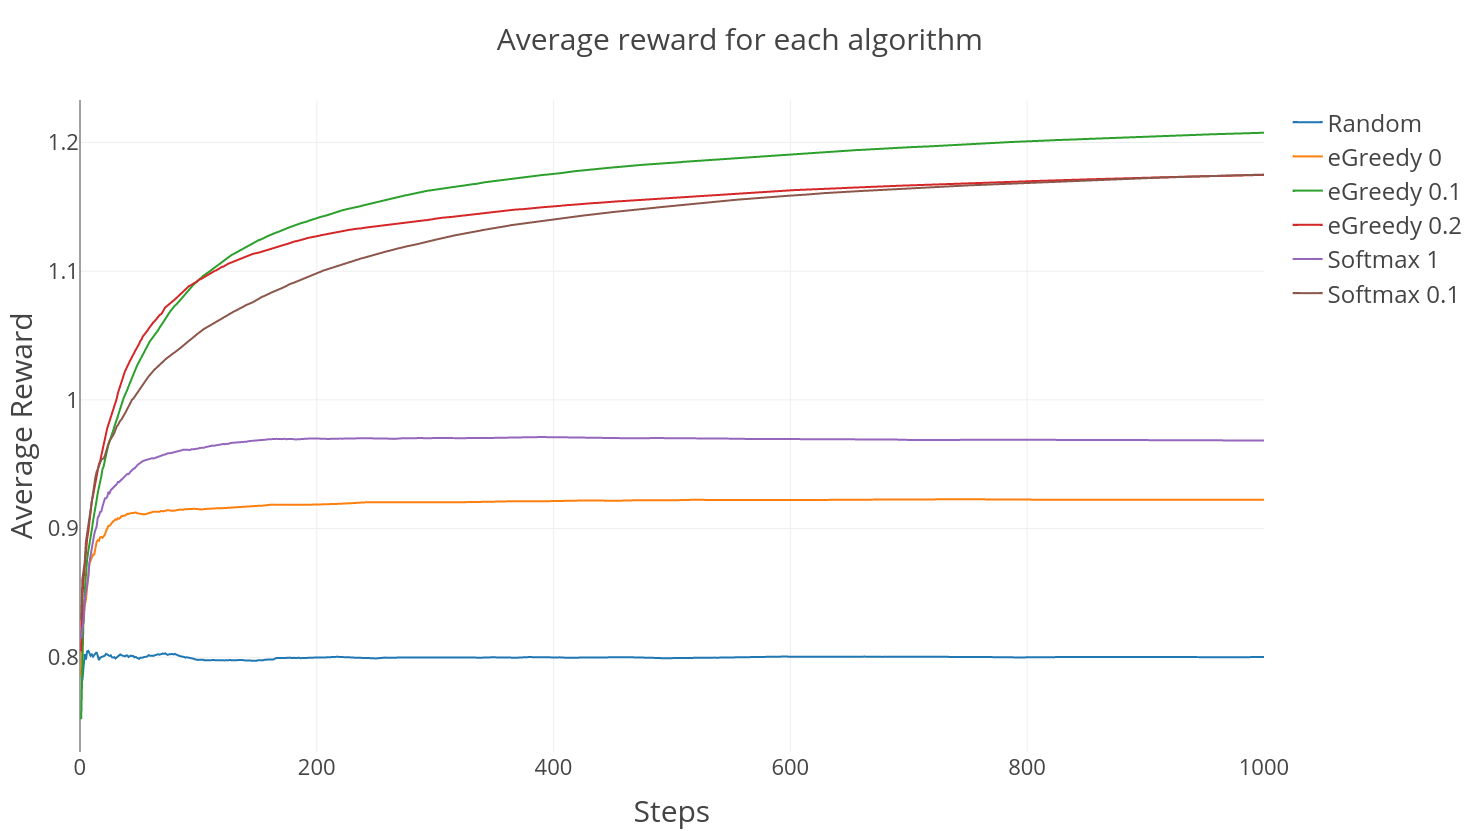
\includegraphics[width=1\linewidth]{ex1_1_average_rewards}
    %\caption{Two Neighborhood types}
\end{figure}

\subsection{Q* values for each arm}

\begin{figure}[H]
	\centering
    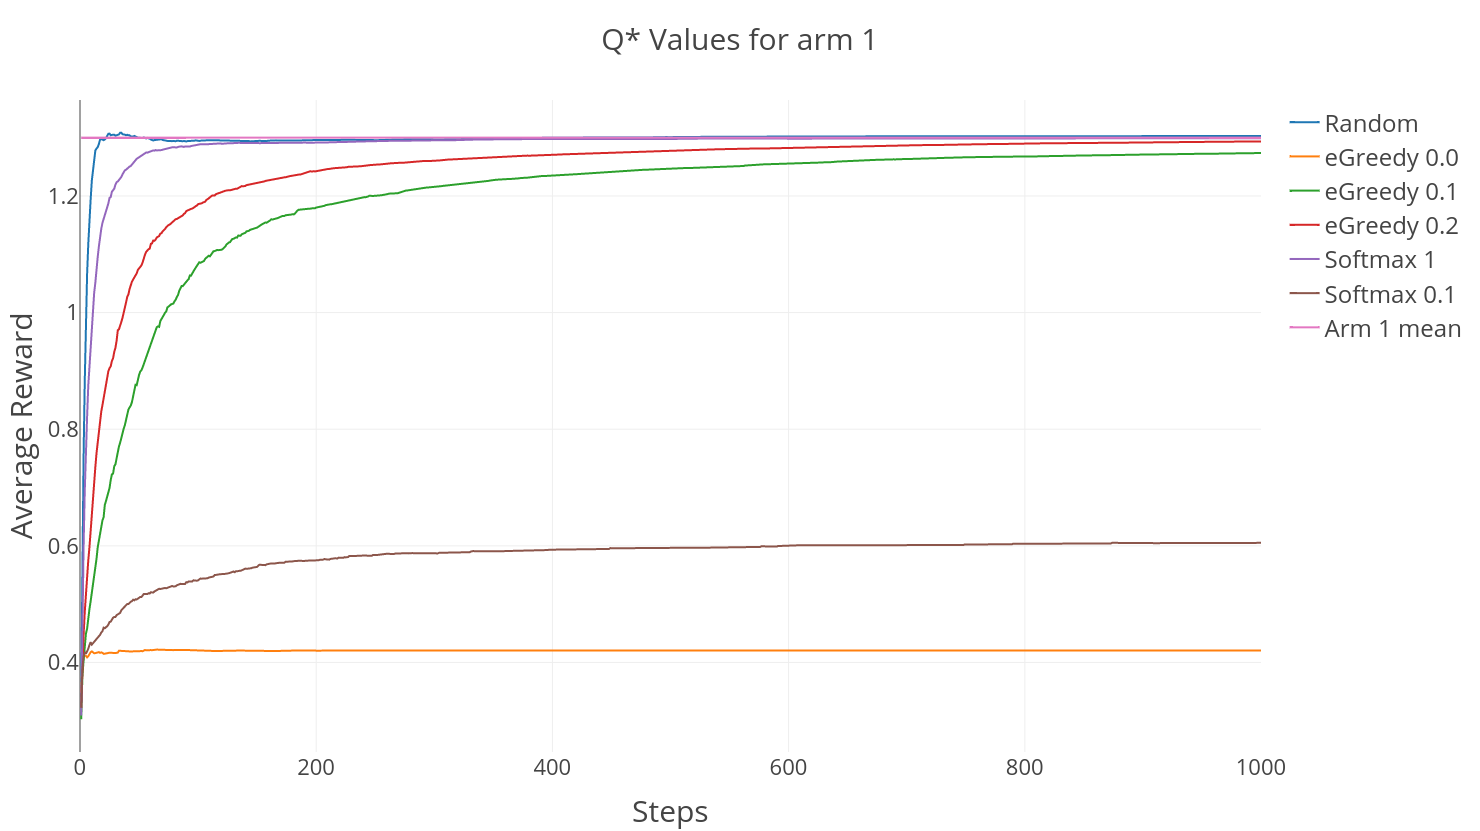
\includegraphics[width=1\linewidth]{ex1_Q1_reward}
    %\caption{Two Neighborhood types}
\end{figure}

\begin{figure}[H]
	\centering
    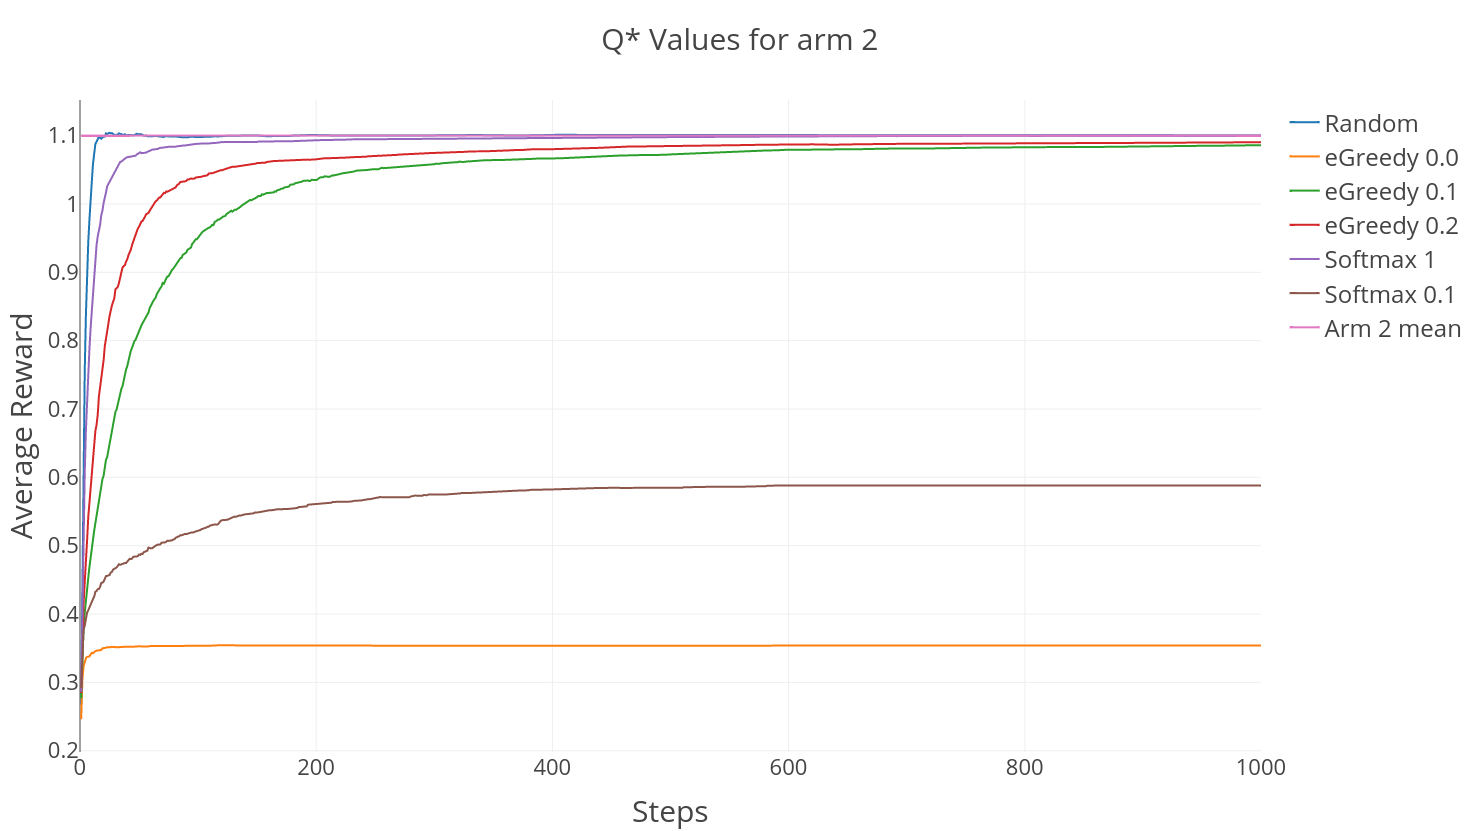
\includegraphics[width=1\linewidth]{ex1_Q2_reward}
    %\caption{Two Neighborhood types}
\end{figure}

\begin{figure}[H]
	\centering
    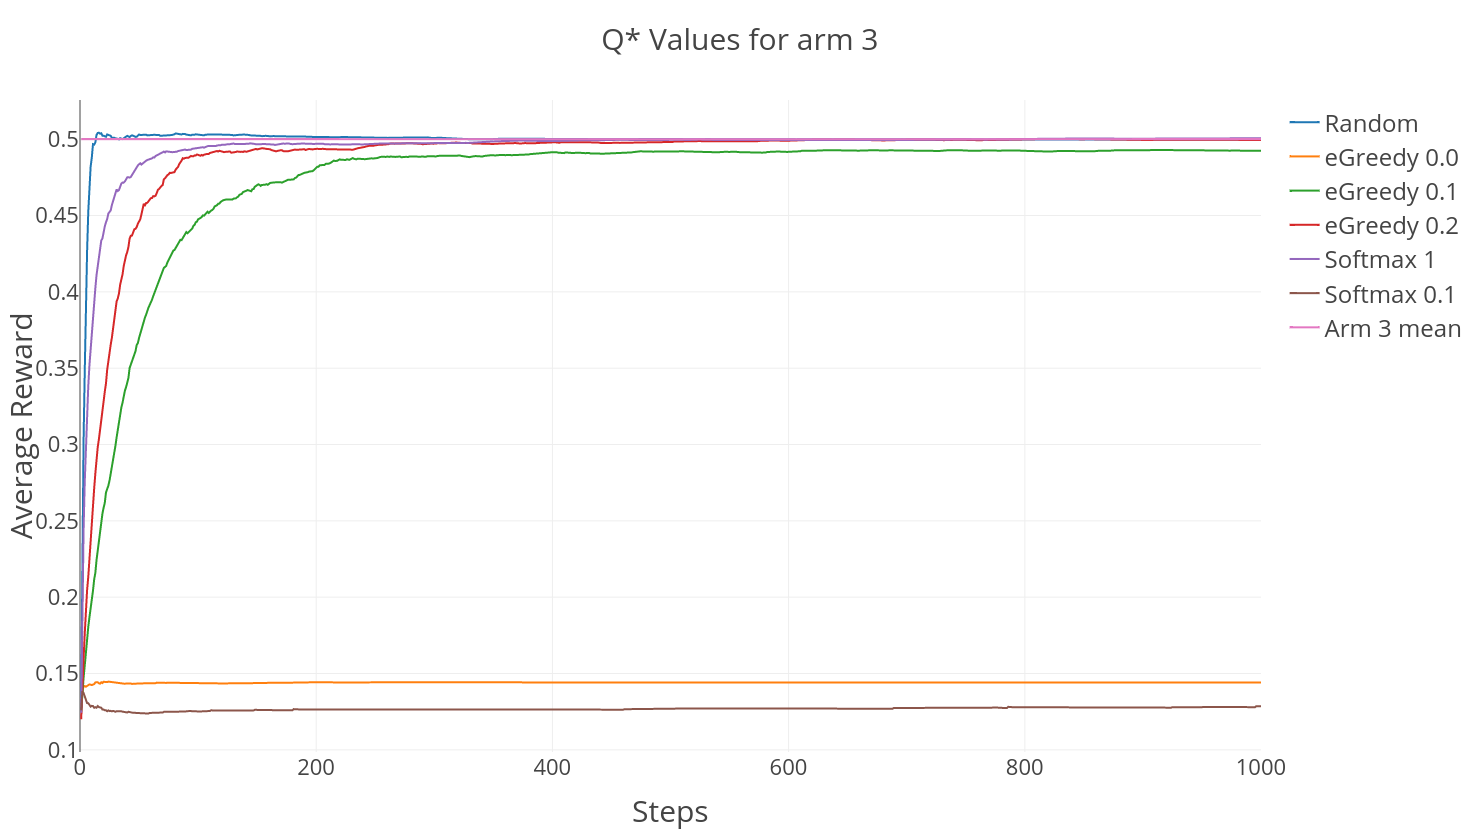
\includegraphics[width=1\linewidth]{ex1_Q3_reward}
    %\caption{Two Neighborhood types}
\end{figure}

\begin{figure}[H]
	\centering
    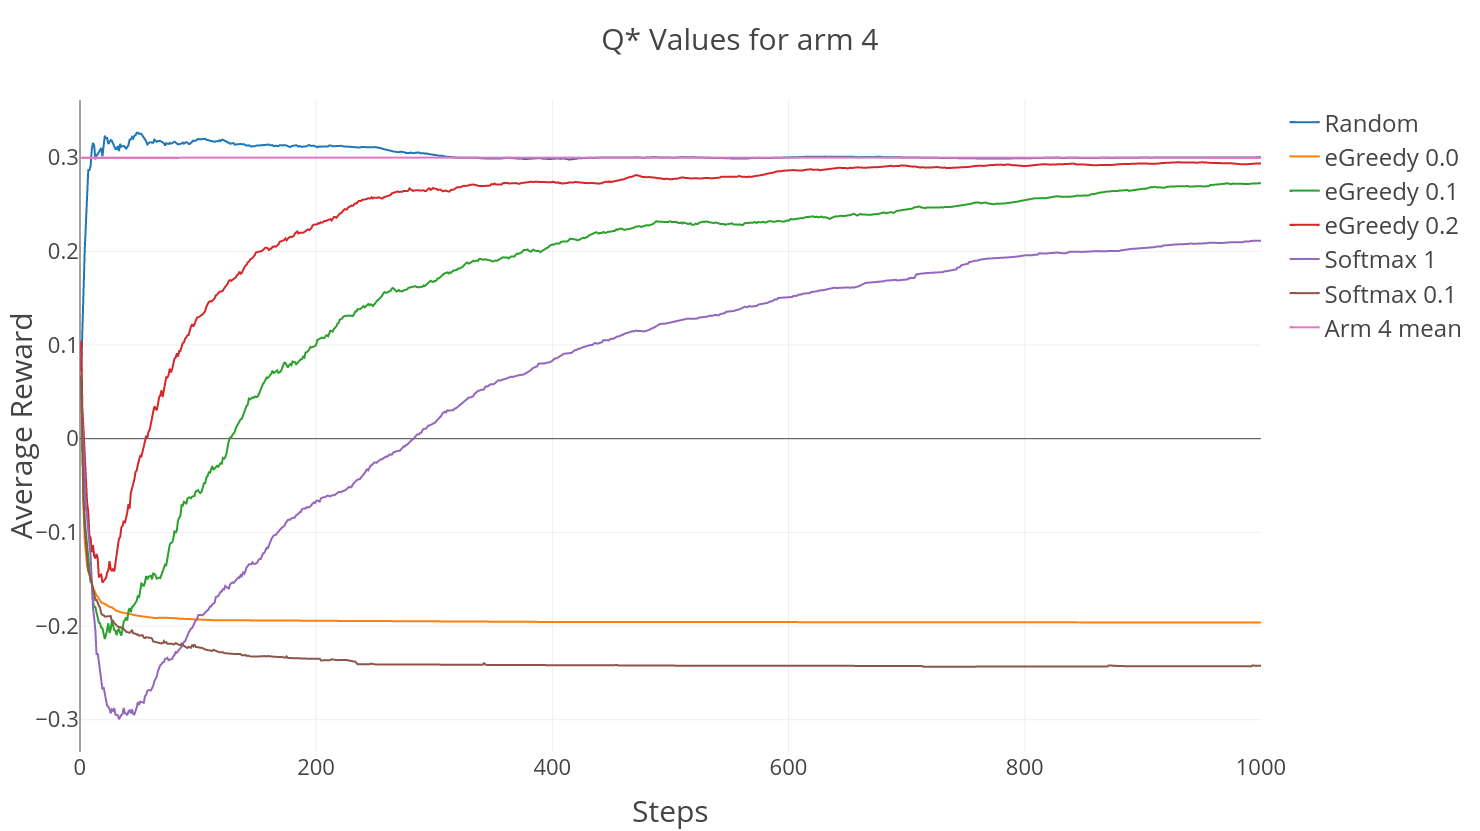
\includegraphics[width=1\linewidth]{ex1_Q4_reward}
    %\caption{Two Neighborhood types}
\end{figure}

\subsection{Histogram on actions chosen}

\begin{figure}[H]
\centering
\begin{subfigure}{.5\textwidth}
  \centering
  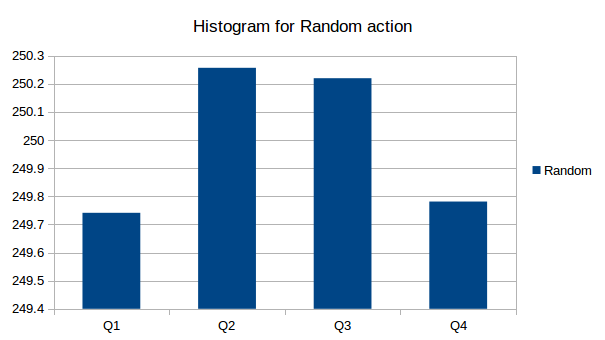
\includegraphics[width=1\linewidth]{ex1_histogram_random}
\end{subfigure}%
\begin{subfigure}{.5\textwidth}
  \centering
  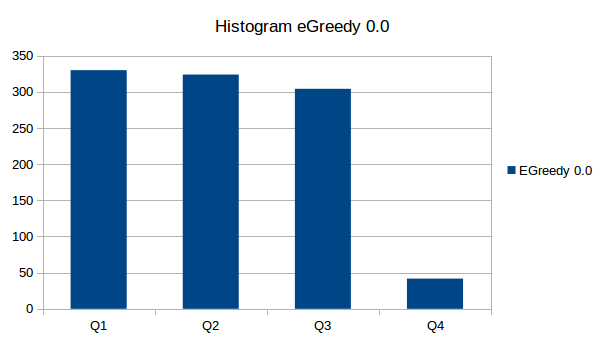
\includegraphics[width=1\linewidth]{ex1_histogram_egreedy00}
\end{subfigure}%

\begin{subfigure}{.5\textwidth}
  \centering
  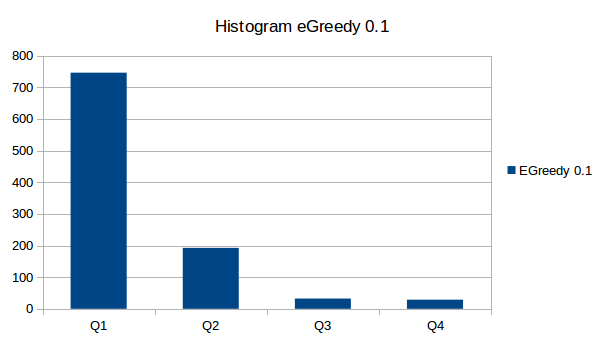
\includegraphics[width=1\linewidth]{ex1_histogram_egreedy01}
\end{subfigure}%
\begin{subfigure}{.5\textwidth}
  \centering
  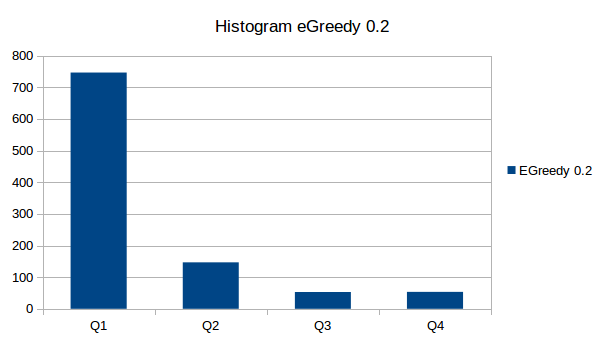
\includegraphics[width=1\linewidth]{ex1_histogram_egreedy02}
\end{subfigure}%

\begin{subfigure}{.5\textwidth}
  \centering
  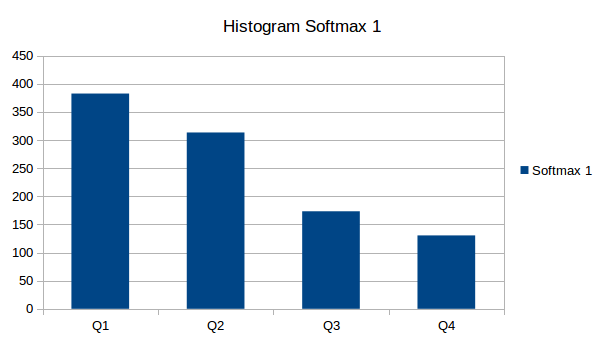
\includegraphics[width=1\linewidth]{ex1_histogram_softmax1}
\end{subfigure}%
\begin{subfigure}{.5\textwidth}
  \centering
  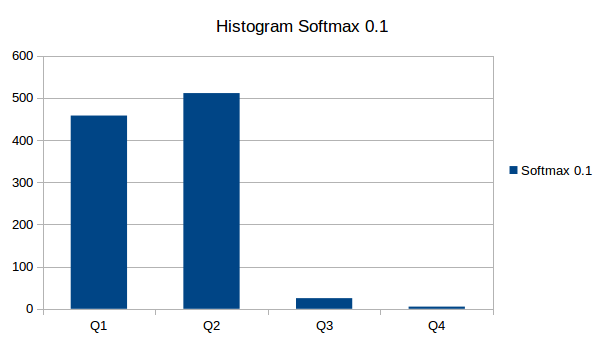
\includegraphics[width=1\linewidth]{ex1_histogram_softmax01}
\end{subfigure}%
\end{figure}


\subsection{Results}

We observe the combined average reward figure: The \textit{eGreedy 0.1} method has the highest average reward after 100 steps until the end of the simulation of 1000 steps. \textit{eGreedy 0.2} and \textit{Softmax 0.1} share the second place together. \textit{Softmax 1} comes in fourth place, \textit{eGreedy 0.0} on fifth and the random algorithm last.

These results can also be observed by looking at the histograms where \textit{eGreedy 0.1} has the highest arm 1 selection.

The random algorithm arrives the fastest at determining the Q* value for every arm but does not yield a good  average. This could indicate that random exploration is a good method in the beginning but has to stop after some steps to select a single arm afterwards to earn the maximum award.

The graphs that show the Q* values for each arm show us that the two methods \textit{eGreedy 0.0} and \textit{Softmax 0.1} are not exploring enough in the beginning as they do not arrive at the actual Q* value and are stuck with a action they selected in the very beginning. This is due to the fact that we are initializing all Q* values to 0 at step 0 which results in the algorithm sticking to one action with a very high percentage without having explored the other actions.

%%%%%%%%%%%%%%%%%%%%%%%%%%%%%%%%%%%%%%%%%%%%%%%%%%%%%%%%%%%%%%%%%%%%%%%%%%%%%%%%
%%%%%%%%%%%%%%%%%%%%%%%%%%%%%%%%%%%%%%%%%%%%%%%%%%%%%%%%%%%%%%%%%%%%%%%%%%%%%%%%
\section{Exercise 2}

\subsection{Combined Average Reward}

\begin{figure}[H]
	\centering
    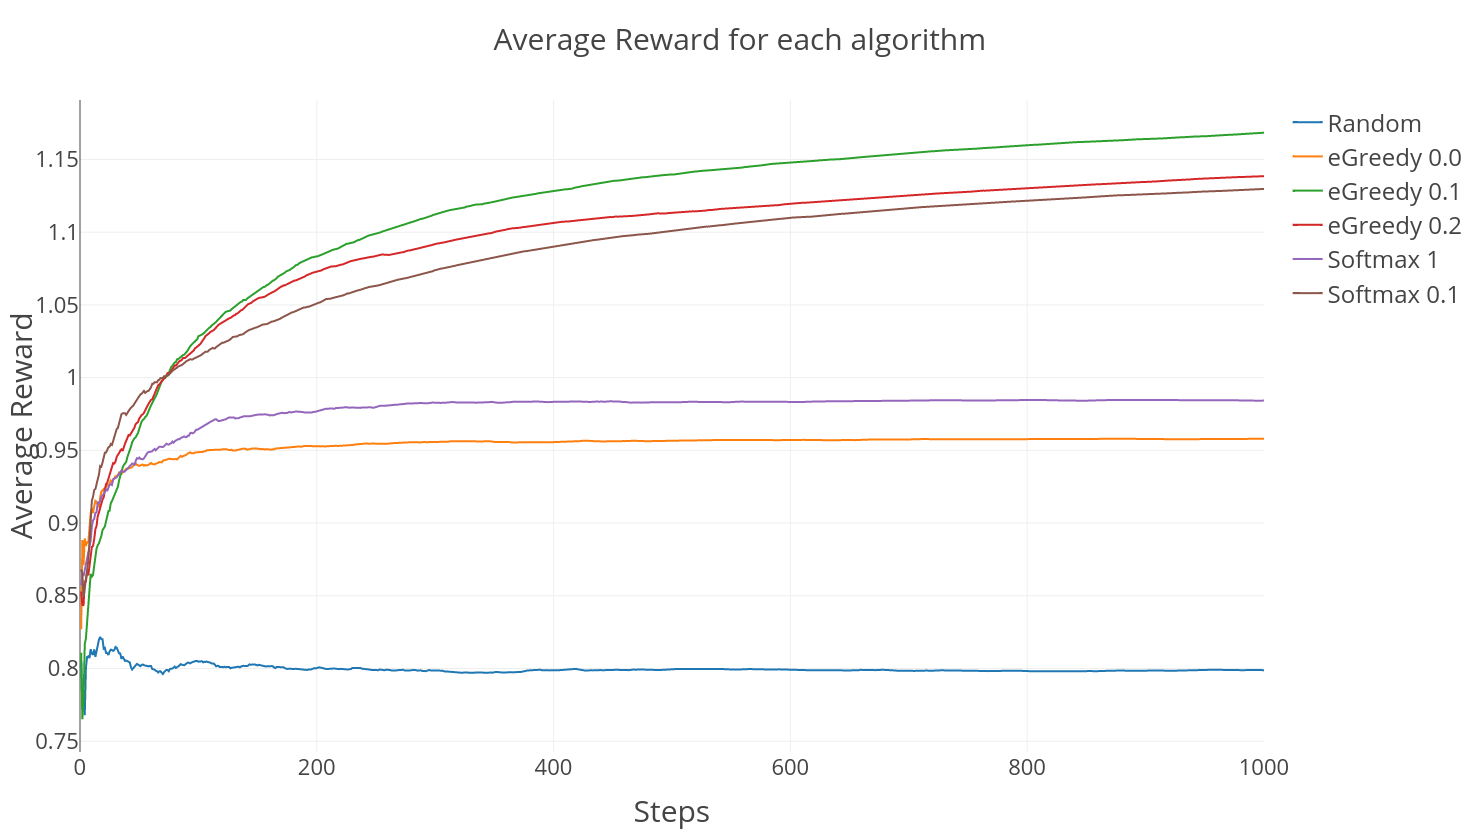
\includegraphics[width=1\linewidth]{ex1_2_average_rewards}
    %\caption{Two Neighborhood types}
\end{figure}

\subsection{Q* values for each arm}

\begin{figure}[H]
	\centering
    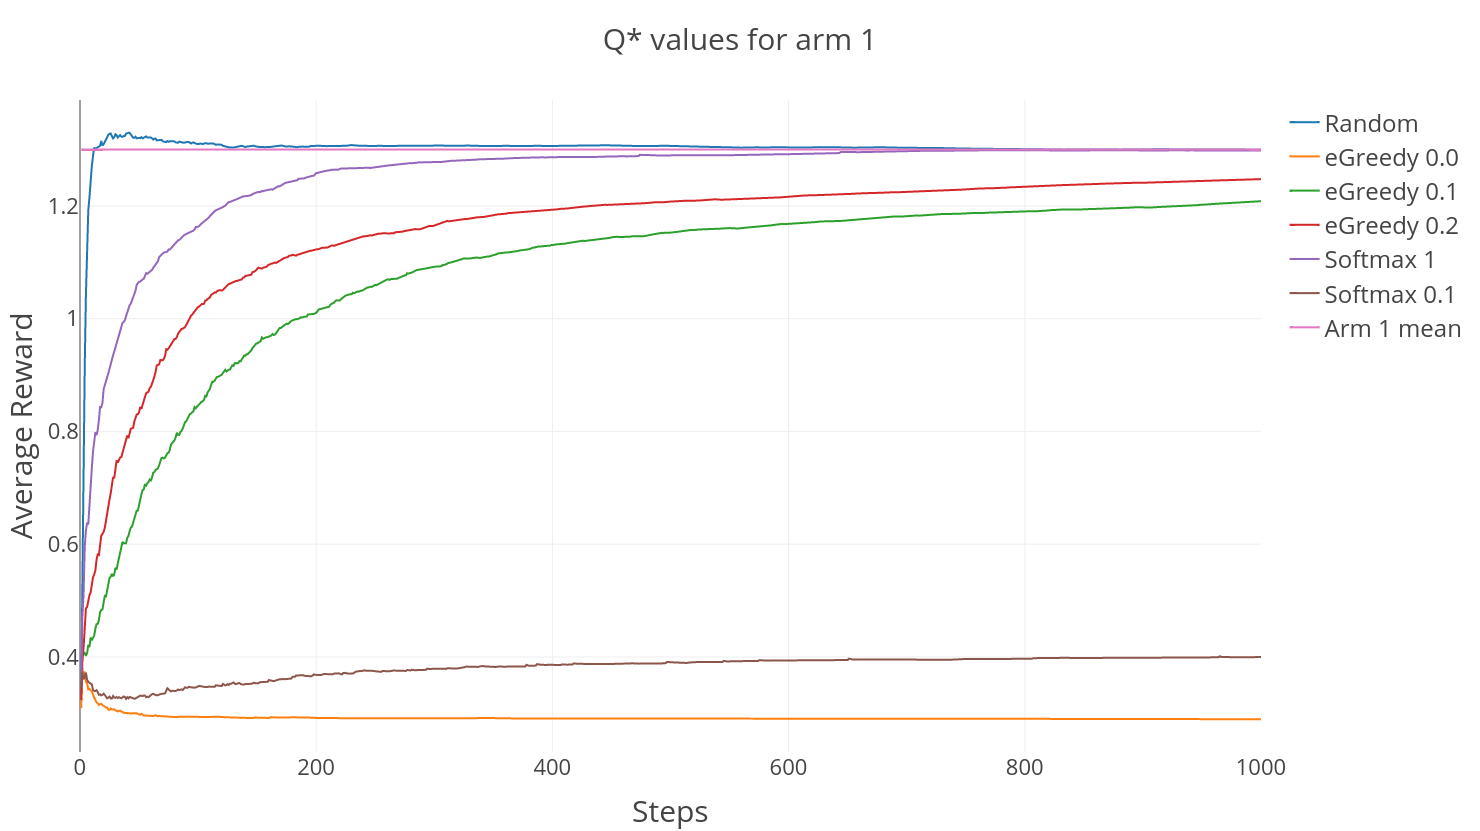
\includegraphics[width=1\linewidth]{ex1_2_Q1_reward}
    %\caption{Two Neighborhood types}
\end{figure}

\begin{figure}[H]
	\centering
    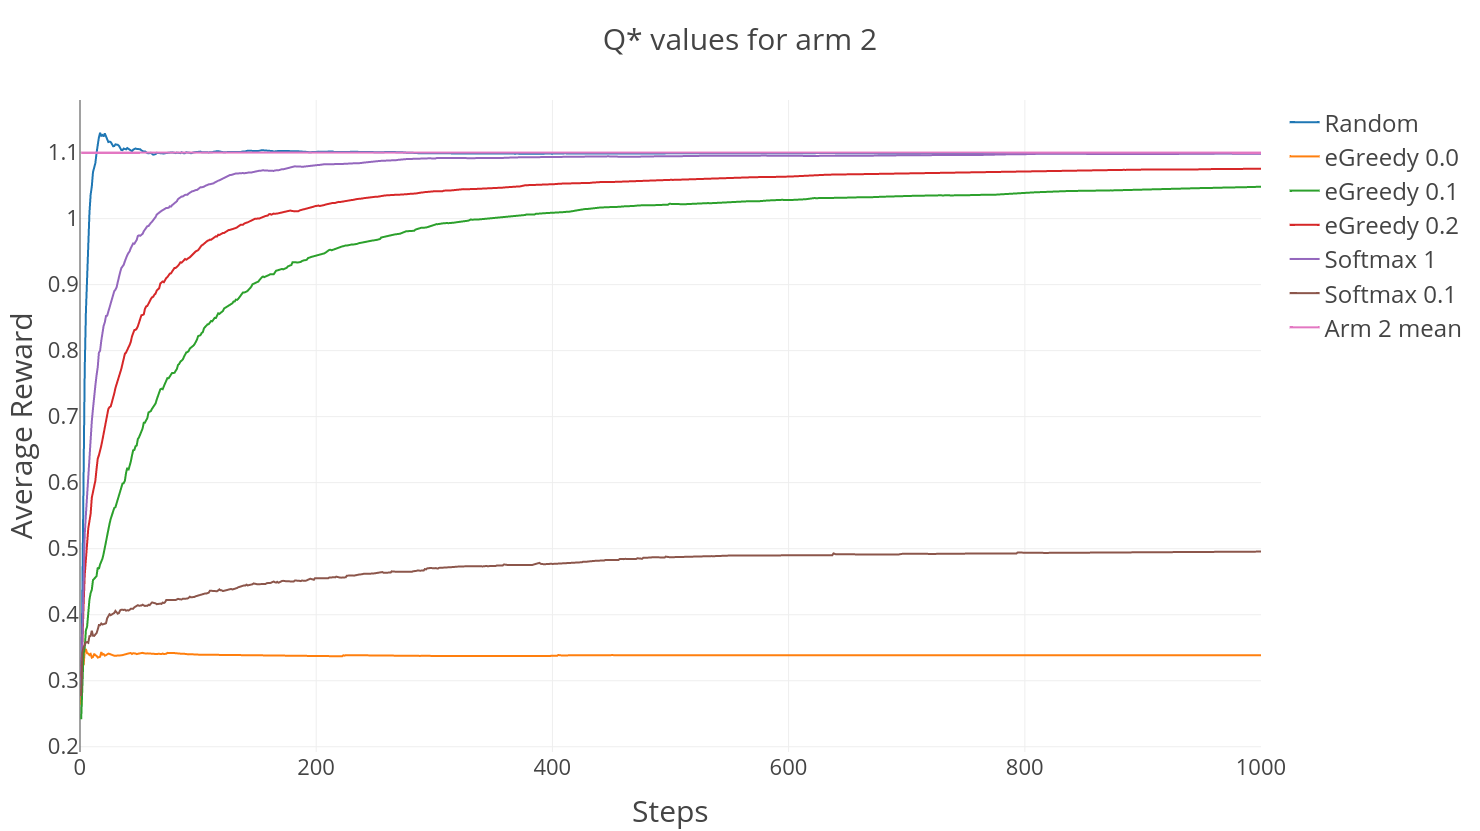
\includegraphics[width=1\linewidth]{ex1_2_Q2_reward}
    %\caption{Two Neighborhood types}
\end{figure}

\begin{figure}[H]
	\centering
    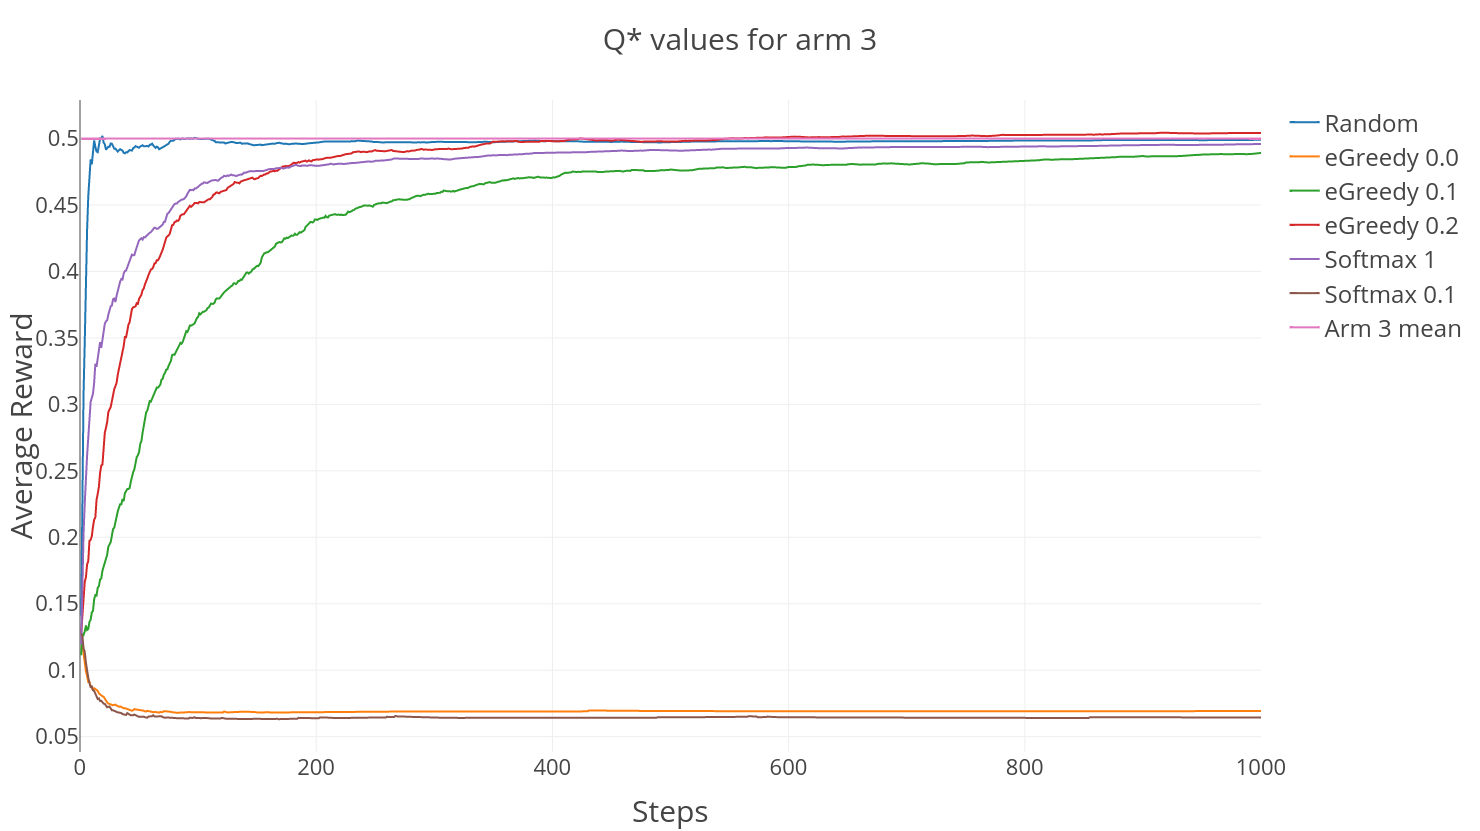
\includegraphics[width=1\linewidth]{ex1_2_Q3_reward}
    %\caption{Two Neighborhood types}
\end{figure}

\begin{figure}[H]
	\centering
    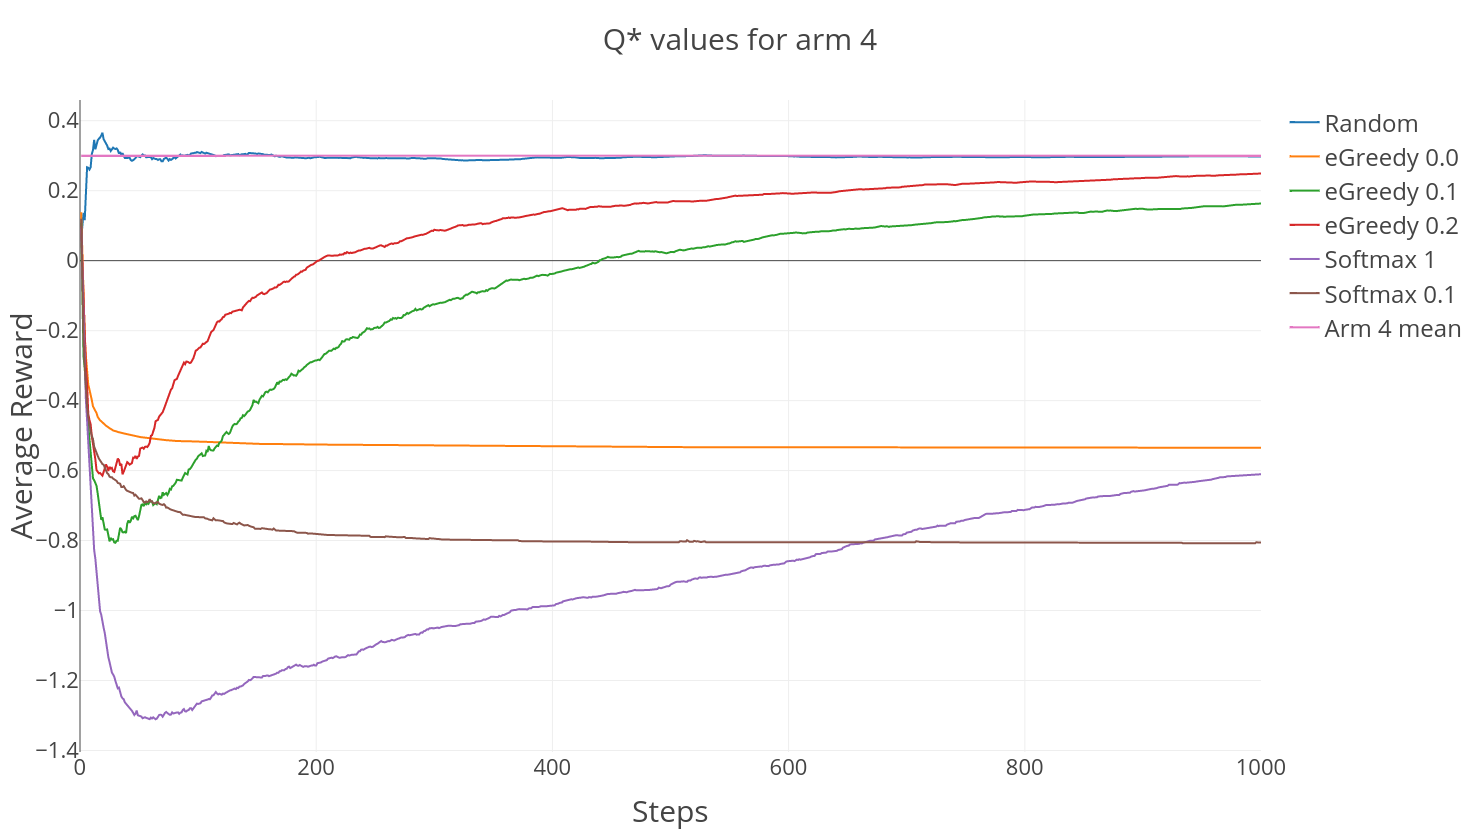
\includegraphics[width=1\linewidth]{ex1_2_Q4_reward}
    %\caption{Two Neighborhood types}
\end{figure}

\subsection{Histogram on actions chosen}

\begin{figure}[H]
\centering
\begin{subfigure}{.5\textwidth}
  \centering
  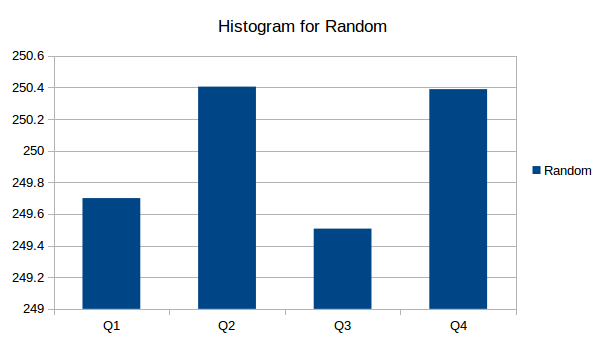
\includegraphics[width=1\linewidth]{ex1_2_histogram_random}
\end{subfigure}%
\begin{subfigure}{.5\textwidth}
  \centering
  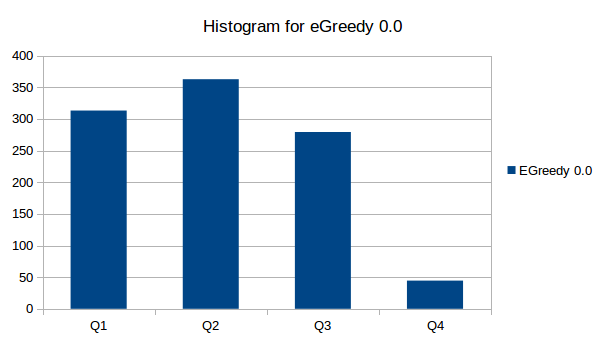
\includegraphics[width=1\linewidth]{ex1_2_histogram_egreedy00}
\end{subfigure}%

\begin{subfigure}{.5\textwidth}
  \centering
  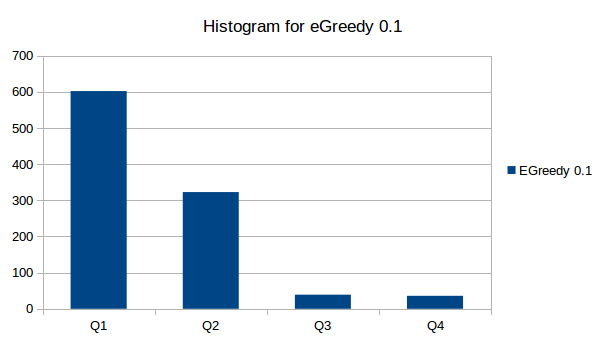
\includegraphics[width=1\linewidth]{ex1_2_histogram_egreedy01}
\end{subfigure}%
\begin{subfigure}{.5\textwidth}
  \centering
  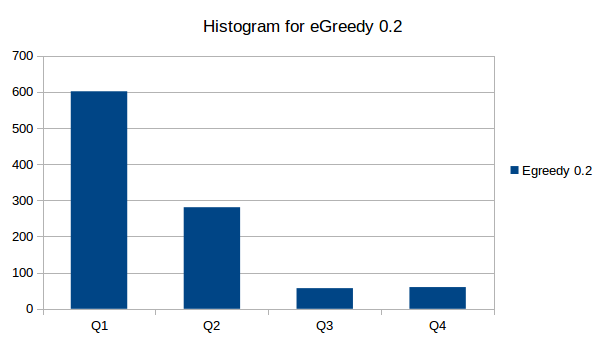
\includegraphics[width=1\linewidth]{ex1_2_histogram_egreedy02}
\end{subfigure}%

\begin{subfigure}{.5\textwidth}
  \centering
  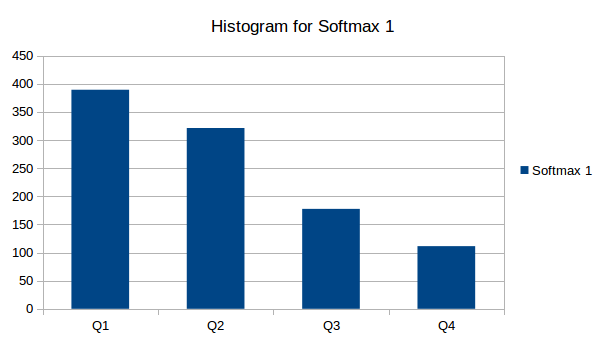
\includegraphics[width=1\linewidth]{ex1_2_histogram_softmax1}
\end{subfigure}%
\begin{subfigure}{.5\textwidth}
  \centering
  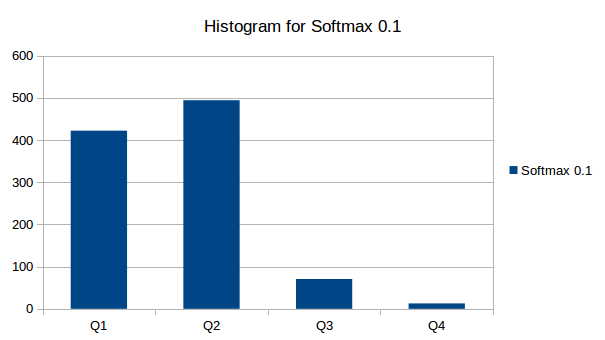
\includegraphics[width=1\linewidth]{ex1_2_histogram_softmax01}
\end{subfigure}%
\end{figure}

\subsection{Results}


Doubling the deviation does not change the order of best algorithms with 1000 steps. The problem is harder to learn as the Q* values are similar to exercise one, but they are doing so with more steps.

The performance, or total reward after 1000 steps influences the used algorithms differently. It decreases the reward for the \textit{eGreedy 0.1} and \textit{eGreedy 0.2} methods but increases the reward slightly for the \textit{Softmax 0.1} method.


The average reward per algorithm is lower than compared to the first exercise. This can be explained due to the fact that the doubling of the deviation makes the Q* values more \textit{random} and hence influences the probability of lower performing arms to be chosen in the beginning.



%%%%%%%%%%%%%%%%%%%%%%%%%%%%%%%%%%%%%%%%%%%%%%%%%%%%%%%%%%%%
\section{Exercise 3}
\subsection{Combined Average Reward}

\begin{figure}[H]
	\centering
    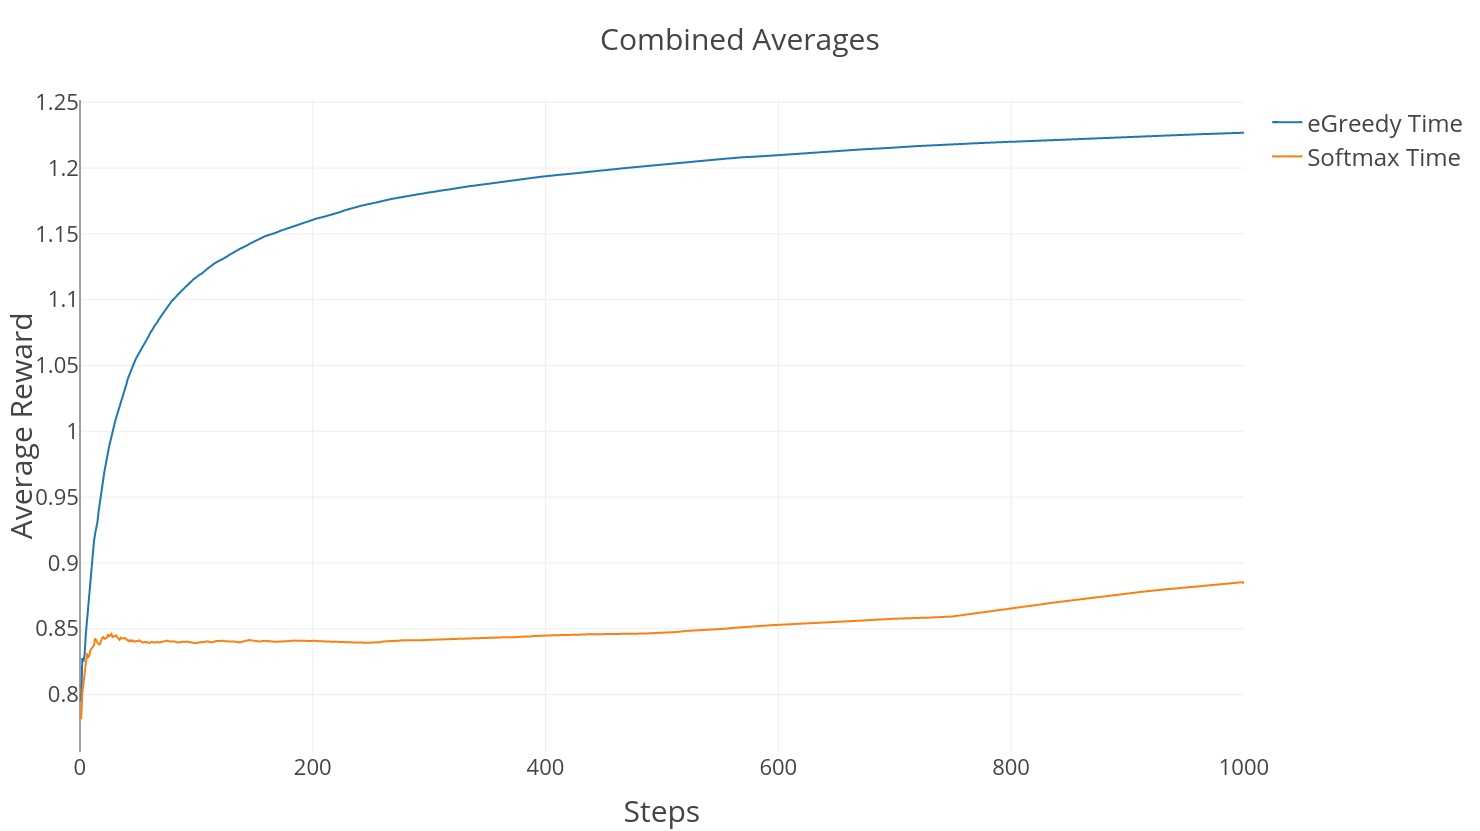
\includegraphics[width=1\linewidth]{ex1_3_average_rewards}
    %\caption{Two Neighborhood types}
\end{figure}

\subsection{Q* values for each arm}

\begin{figure}[H]
	\centering
    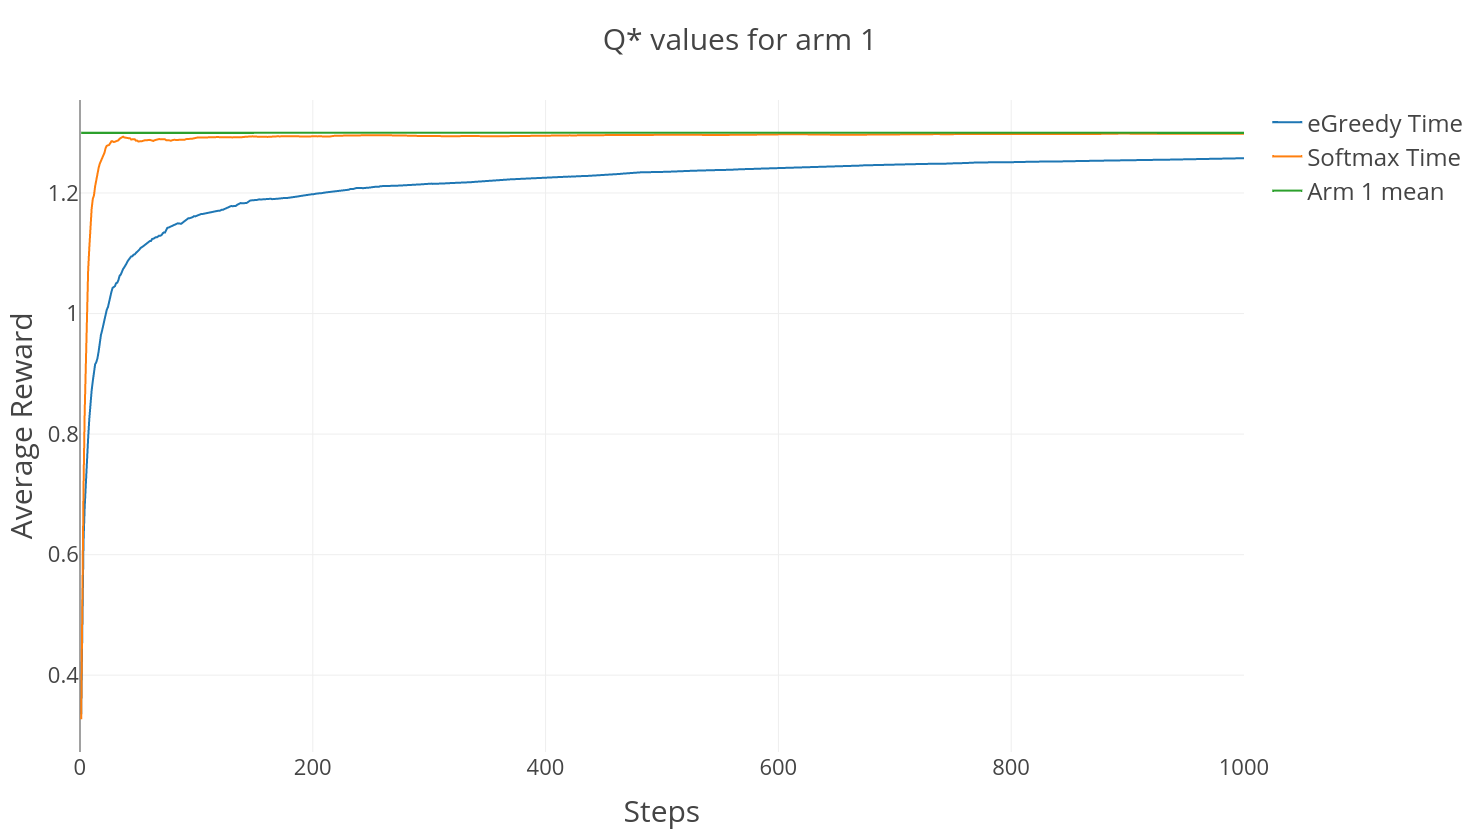
\includegraphics[width=1\linewidth]{ex1_3_Q1}
    %\caption{Two Neighborhood types}
\end{figure}

\begin{figure}[H]
	\centering
    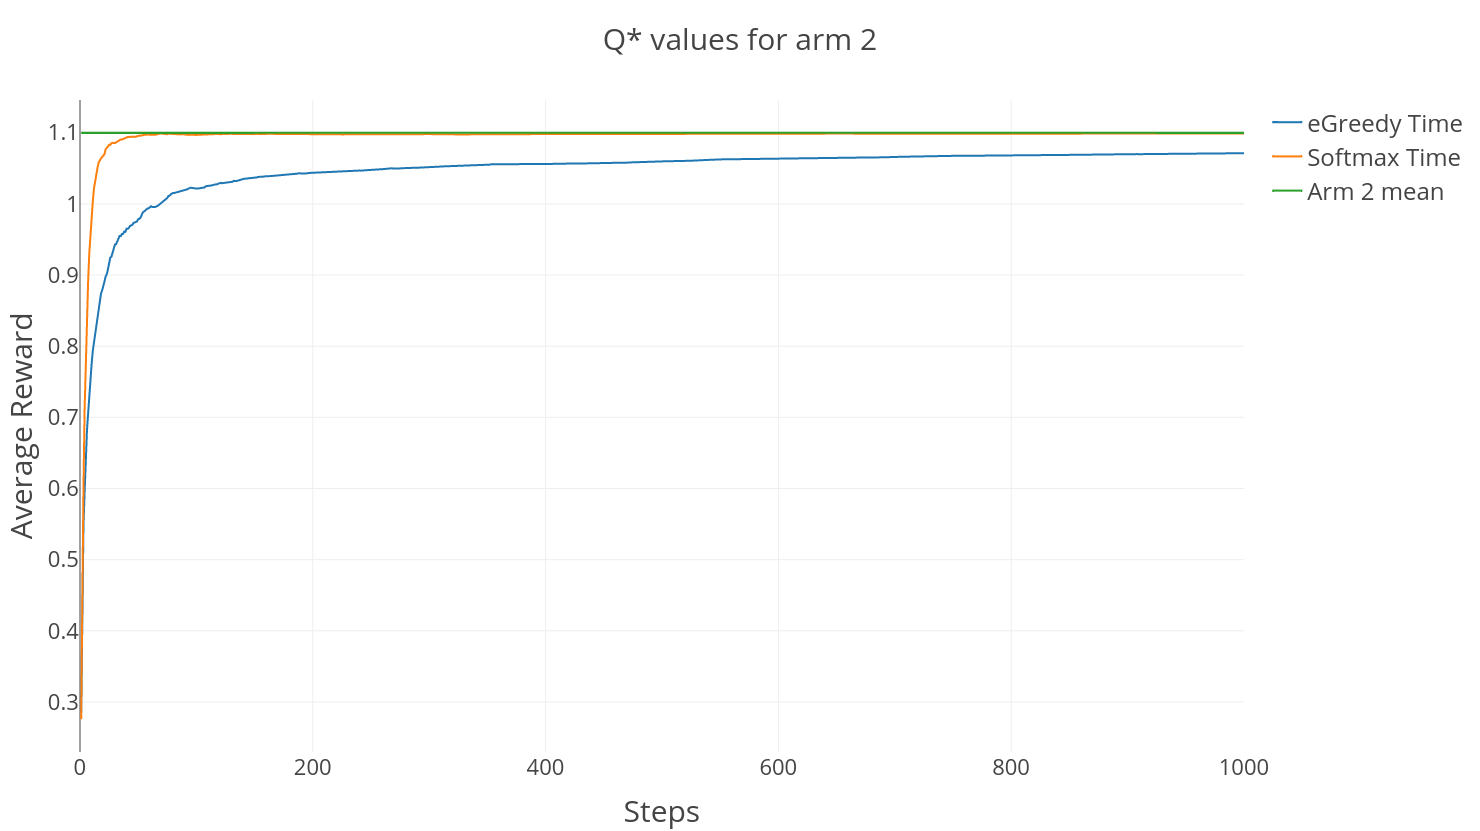
\includegraphics[width=1\linewidth]{ex1_3_Q2}
    %\caption{Two Neighborhood types}
\end{figure}

\begin{figure}[H]
	\centering
    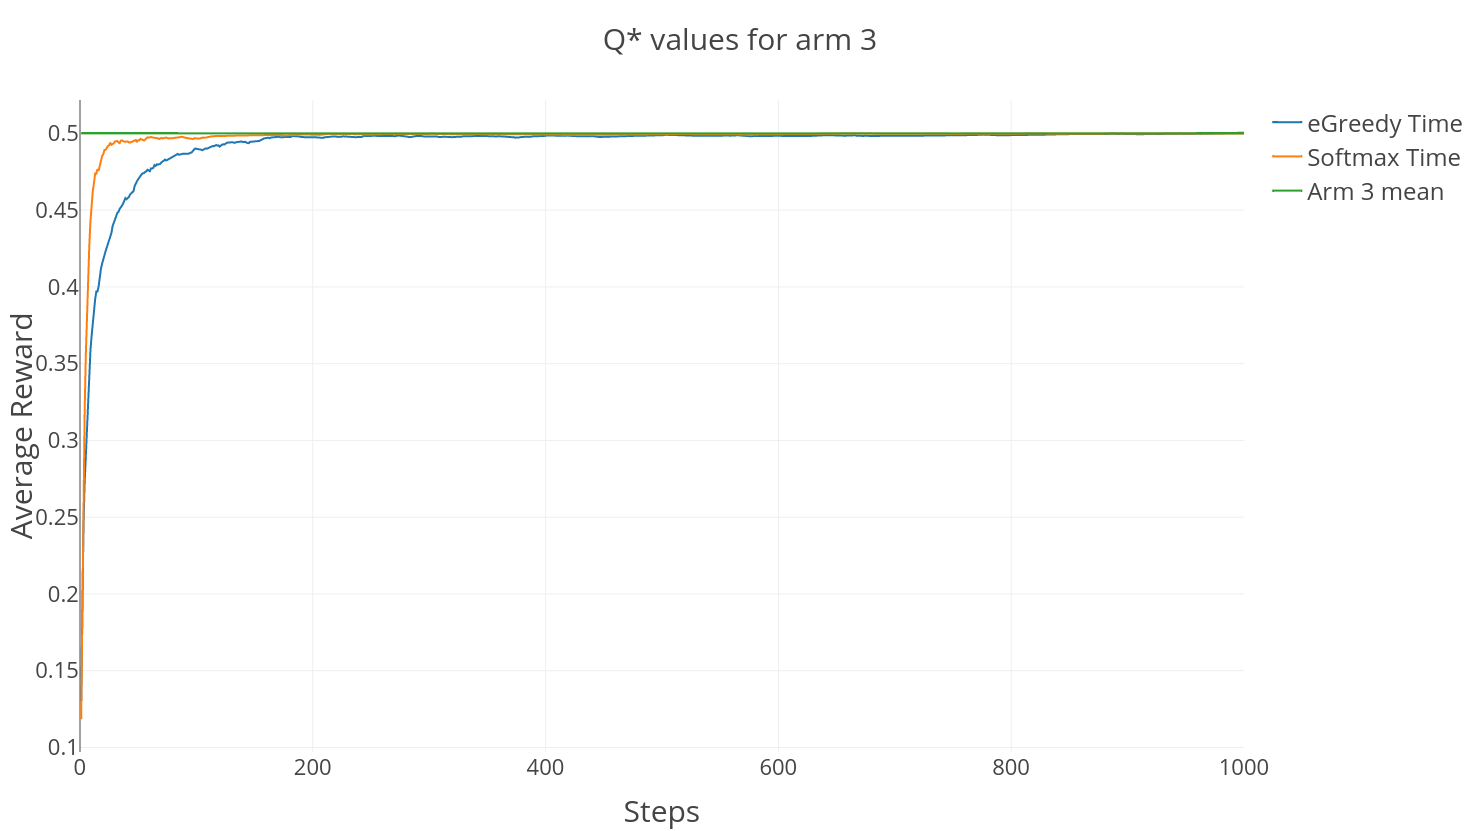
\includegraphics[width=1\linewidth]{ex1_3_Q3}
    %\caption{Two Neighborhood types}
\end{figure}

\begin{figure}[H]
	\centering
    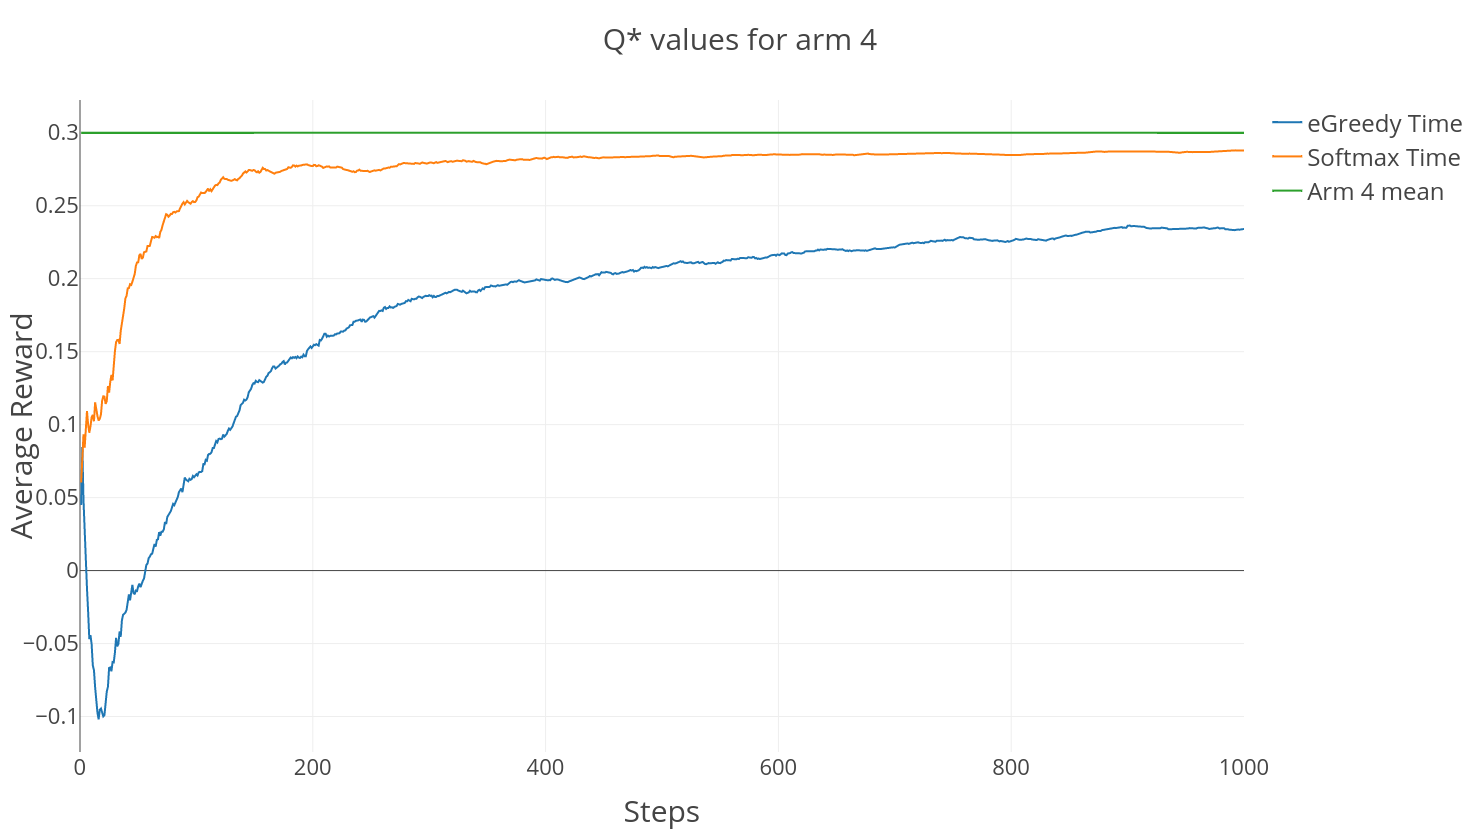
\includegraphics[width=1\linewidth]{ex1_3_Q4}
    %\caption{Two Neighborhood types}
\end{figure}

\subsection{Histogram on actions chosen}

\begin{figure}[H]
\centering
\begin{subfigure}{.5\textwidth}
  \centering
  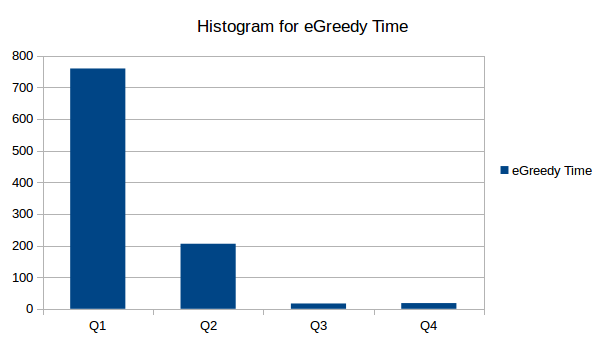
\includegraphics[width=1\linewidth]{ex1_3_histogram_egreedytime}
\end{subfigure}%
\begin{subfigure}{.5\textwidth}
  \centering
  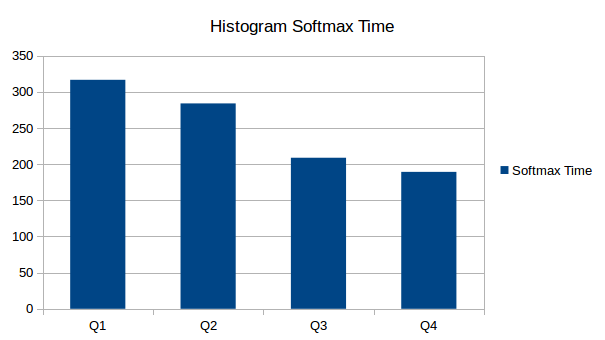
\includegraphics[width=1\linewidth]{ex1_3_histogram_softmaxtime}
\end{subfigure}%
\end{figure}

\subsection{Results}

The new \textit{eGreedy} algorithm performs better than any other algorithm. The new \textit{Softmax} algorithm performs only better than the \textit{random} algorithm after 1000 time steps but has an increasing curve. Over a longer time-period, it would out-perform the bottom three algorithms - \textit{Random}, \textit{eGreedy 0.0} and \textit{Softmax 1}.

From the Q* value graphs we can observe that the \textit{Softmax Time} method is able to find the mean value of each arm faster than the \textit{eGreedy Time} method due to its higher exploration at the beginning. It does not outperform it though, as it exploits the best arm later.

We can conclude from these experiments that the best way to achieve the highest reward over time is to explore at the beginning and then only exploit after some time. The downside of the \textit{eGreedy} algorithms is that they keep exploring even though they already \textit{learned} the best arms.


\newpage
\section{Stochastic Reward Game}

The three cases were simulated 100 times each and their results averaged. This is necessary due to the biased nature of the Boltzmann selection algorithm.

\subsection{Plotting}
\begin{figure}[H]
	\centering
	\caption{a) $\sigma_0 = \sigma_1 = \sigma = 0.2$}
    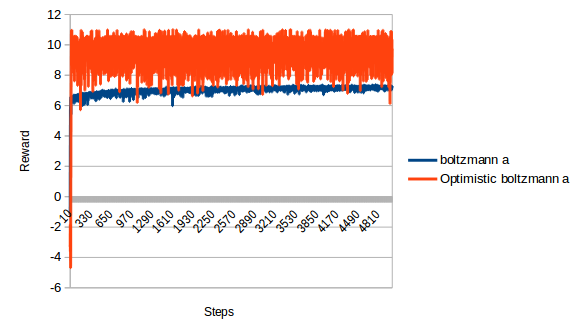
\includegraphics[width=1\linewidth]{ex2_a}
\end{figure}

\begin{figure}[H]
	\centering
	\caption{b) $\sigma_0 = 4$, $\sigma_1 = \sigma = 0.1$}
    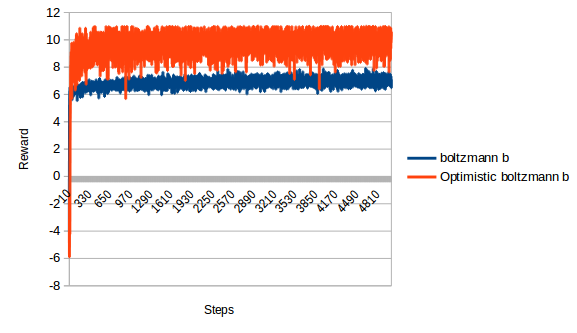
\includegraphics[width=1\linewidth]{ex2_b}
\end{figure}

\begin{figure}[H]
	\centering
	\caption{c) $\sigma_1 = 4$, $\sigma_0 = \sigma = 0.1$}
    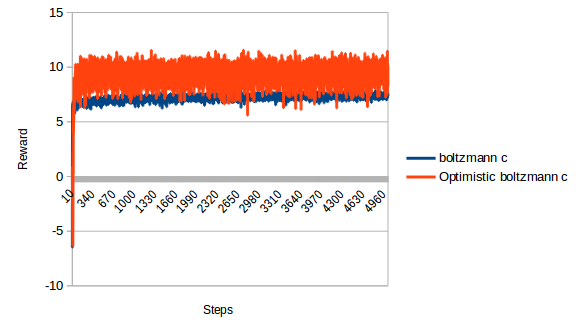
\includegraphics[width=1\linewidth]{ex2_c}
\end{figure}

For all of the three cases, the Optimistic Boltzmann algorithm performs better than the simple Boltzmann algorithm. In the first few steps we can see the optimistic Boltzmann algorithm exploring the estimates which is why it starts off negatively. The standard Boltzmann algorithm also starts off negatively, but only for the first round. It reaches the non-optimal strategy of $<a2,b2>$ in every of the three cases. The optimistic strategy finds for the most case the optimal strategy of $<a1,b1>$. It has a far higher deviation, even with 100 simulations, meaning that it still sometimes chooses the action of $<a2,b2>$. This could be reduced to obtain a pure $<a1,b1>$ action with a decreasing temperature.


\subsection{Discussion}

\subsubsection{Changing the learning process to independent learners}

Changing to independent learners means that they do not observe of action played by the opposing player. This be the same as the n-armed bandit problem but with multiple distributions for each action. A independent learner would behave the same as the simple Boltzmann selection but would converge to the $<a2,b2>$ action slower. The research done by \textit{Caroline Claus and Craig Boutilier}\cite{Claus:1998:DRL:295240.295800} confirm this behaviour. They also show that the higher the penalty in the field $<a1,b2>$ and $<a2,b1>$, the lower the chance of converging to the optimal action. 

\subsubsection{Always selecting highest reward}
Assuming both players keep knowledge of every joint action and their rewards and that not played actions are given a very high reward so that exploring can occur, they will converge fast to a joint action. This is not necessarily the best action, as the exploration is minimal and their estimates of each action might not be close to the mean. Taking our example, if they explore the field $<a1,b1>$ once and it yields a reward of 5 due to a high deviation, they will play other actions, assuming they have previously explored some other actions which yielded a higher reward than 5. Meaning that the low exploration of this technique means that the best action might not be chosen.
 


%%%%%%%%%%%%%%%%%%%%%%%%%%%%%%%%%%%%%%%%%%%%%%%%%%%%%%%%%%%%%%%%%%%%%%%%%
%% Bibliography start
\newpage

\bibliographystyle{unsrt}
\bibliography{bibliography}


\end{document}